%%%%%%%%%%%%%%%%%%%%%%%%%%%%%%%%%%%%%%%%%
% Stylish Article
% LaTeX Template
% Version 2.1 (1/10/15)
%
% This template has been downloaded from:
% http://www.LaTeXTemplates.com
%
% Original author:
% Mathias Legrand (legrand.mathias@gmail.com)
% With extensive modifications by:
% Vel (vel@latextemplates.com)
%
% License:
% CC BY-NC-SA 3.0 (http://creativecommons.org/licenses/by-nc-sa/3.0/)
%
%%%%%%%%%%%%%%%%%%%%%%%%%%%%%%%%%%%%%%%%%

%----------------------------------------------------------------------------------------
%	PACKAGES AND OTHER DOCUMENT CONFIGURATIONS
%----------------------------------------------------------------------------------------

\documentclass[fleqn,10pt]{SelfArx} % Document font size and equations flushed left

\usepackage[english]{babel} % Specify a different language here - english by default

\usepackage{lipsum} % Required to insert dummy text. To be removed otherwise

%----------------------------------------------------------------------------------------
%	COLUMNS
%----------------------------------------------------------------------------------------

\setlength{\columnsep}{0.55cm} % Distance between the two columns of text
\setlength{\fboxrule}{0.75pt} % Width of the border around the abstract

%----------------------------------------------------------------------------------------
%	COLORS
%----------------------------------------------------------------------------------------

\definecolor{color1}{RGB}{0,0,90} % Color of the article title and sections
\definecolor{color2}{RGB}{0,20,20} % Color of the boxes behind the abstract and headings

%----------------------------------------------------------------------------------------
%	HYPERLINKS
%----------------------------------------------------------------------------------------

\usepackage{hyperref} % Required for hyperlinks
\hypersetup{hidelinks,colorlinks,breaklinks=true,urlcolor=color2,citecolor=color1,linkcolor=color1,bookmarksopen=false,pdftitle={Title},pdfauthor={Author}}

%----------------------------------------------------------------------------------------
%	ARTICLE INFORMATION
%----------------------------------------------------------------------------------------

\JournalInfo{Data Mining B565 Fall 2016} % Journal information
\Archive{ALL WORK HEREIN IS OURS!} % Additional notes (e.g. copyright, DOI, review/research article)

\PaperTitle{On the Prediction of User Browsing Interests from Past Navigation Data} % Article title

\Authors{Andrew Patterson, Joo-Wang John Lee, Matthew Schlegel} % Authors
\affiliation{\textit{Computer Science, School of Informatics and Computing, Indiana University, Bloomington, IN, USA}} % Author affiliation

\affiliation{\{jl216,andnpatt,mkschleg\}@indiana.edu} % Corresponding author

\Keywords{Regression --- House Sale Prices --- Data Mining} % Keywords - if you don't want any simply remove all the text between the curly brackets
\newcommand{\keywordname}{Keywords} % Defines the keywords heading name

%----------------------------------------------------------------------------------------
%	ABSTRACT
%----------------------------------------------------------------------------------------

\Abstract{The prediction of users’ interests in web browsing has been a burgeoning area of research in data mining.  Analyzing past user navigation data, discovering trends on key topics searched on by a user has many applications and benefits in easing browsing of the internet. The online advertisting company, Outbrain provides a vast amount of navigation data including time stamps, the method through which the links were accessed, and ad links clicked.  Using this large dataset, this paper explores a couple of different methods including maximum likelihood estimation and neural networks to analyze the data and make predictions on expected user behavior.}

%----------------------------------------------------------------------------------------

\begin{document}

\flushbottom % Makes all text pages the same height

\maketitle % Print the title and abstract box

\tableofcontents % Print the contents section

\thispagestyle{empty} % Removes page numbering from the first page

%----------------------------------------------------------------------------------------
%	ARTICLE CONTENTS
%----------------------------------------------------------------------------------------

\section*{Introduction} % The \section*{} command stops section numbering

\addcontentsline{toc}{section}{Introduction} % Adds this section to the table of contents

The internet has grown significantly in size and depth in its years of use by the average user. From this growth the interesting and difficult problem of predicting a user’s behavior and preferences has become important to many businesses and websites. Websites want to produce and serve content and ads that a user will click, and large businesses and news organizations such as Amazon, CNN, and the New York Times want to keep users within the scope of their content to increase views and ad revenue. On the other side, users want content to be easily accessible and to be curated towards their interests.

Outbrain is a company that handles the complex task of content curation for individual users.  Using data gathered through their online portals, the key problem is to build a system to predict whether a user will click an ad based on the content of their previous page visits. More specifically, leveraging the similarities between user history of visited webpages and content preferences would help accurately predict what users will want to visit next, and to also curate content to improve user experience and possible ad revenue.

The dataset provided from Outbrain is large and complex. It includes information on user’s page views, and the content of each of the pages viewed by a user. There is a temporal feature that could allow for the model to take advantage of temporal trajectories of web habits, location information to inform whether the user’s views are influenced on location, and what type of platform they are using to view the web content. There is also information about the documents viewed such as content type and publisher. For simplicity, the content of the document, specifically the category and topics, was decided as the key factor considered in collecting data on user views. The temporal and location information in our preliminary work was ignored as it is not obvious how to incorporate this information for this project and it adds significant complexity.

The first step is to use a matrix factorization of the users cross pageviews. From this, the angle between users can be calculated to find similar candidates. This data can also be used to “cluster” users based on pageviews to find the probability that this group of user has clicked this data point. Because the set is so big there is an increased interest in computationally efficient algorithms.

%------------------------------------------------

\section{Background}

Previously many approaches have been taken to solve the click through rate (CTR) prediction problem.
Microsoft has used a sparse logistic regression approach over a set of hand crafted features. These features include the log number of characters in the title, the predicted category, or the most commonly used word (with stopping words) in the ad \cite{richardson2007predicting}. Microsoft has also provided a handful of baselines to compare multiple document features for the CTR problem and has found that the Bag of Words methods work incredibly well using probit models and naive bayes classifiers \cite{graepel2010web}.

Microsoft researchers have experimented with Bayesian Networks for CTR prediction. General Click Model (GCM) is a Dynamic Bayesian Network which attempts to model the probability of an ad being clicked in a similar way as naive bayes. The condition of independence between features is lessened than with naive bayes by allowing a structurally dynamic network to learn the condition dependence of features resulting in a more general model \cite{zhu2010novel}.

Yahoo researchers have used Poisson prior probability distributions to model the CTR based on location and time features. They compared this model to a sparsity inducing linear regression model on the same features \cite{agarwal2009spatio}. This approach seems particularly limited as spatial features tend to be based on improper priors. In fact, most methods using spatial features manage to learn something akin to a population density graph based on location, which is perhaps not particularly meaningful for the CTR problem. Other researchers at Yahoo utilized user click history to determine the probability of a new user clicking an ad. They attempted their method on a handful of prediction algorithms: Maximum Entropy, Adaboost, and Gradient Boosting Decision Trees. None of the models worked \cite{hillard2010improving}.

Finally Google has developed CTR prediction methods based only on click history using Contextual Multi-arm Bandit algorithms to model the probability of individual ads being clicked \cite{lu2010contextual}.

There is a considerable amount of work attempting to solve the problem of CTR prediction. One of the major drawbacks is the massive amount of data involved. \cite{mcmahan2013ad} discusses many of the problems related to feature engineering when selecting models. They identify many ways to reduce the number of bits necessary to model simple details like document categorization and topic. They further discuss using simple models like Follow the Regularized Leader (FTRL-Proximal) which is globally convex and easy to train, and spending more time discovering the important features behind CTR prediction.

There seems to be a trend in CTR research towards using much simpler models as opposed to the deep learning or related models found in other parts of the machine learning community.

%------------------------------------------------

\section{Algorithm and Methodology}

% We used two models to predict CTR. First we used a very simplistic model that approximates the Maximum Likelihood Estimate of the probability of each ad being clicked given click history. This model needed no data preparation. We added a regularization term to the model to prevent overfitting given the size of the click history. The model looks like:

The first model that was tested was a Maximum Likelihood Estimate of $p(click|history of clicks)$ with a regularization term to prevent overfitting. The model is calculated via

% \begin{center}
\begin{eqnarray}
    \hspace{0.3in}p(click) &=& \frac{\sum{c}}{n * (\theta + log(n + \gamma))},
\end{eqnarray}
% \end{center}

where $\sum{c}$ is the number of clicks for a given ad and $n$ is the total number of clicks in the click history. $\theta$ is a regularization weight that pulls the prior probability distribution towards preferring more general solutions and $\gamma$ is used to guarantee the $log(n)$ is defined for all $n$ and thus is set such that $\gamma << n$.

The second model used for CTR prediction was a shallow neural network that mapped a set of category and topic features from the documents to the probability of being clicked. This model used a one-hot (or one in k) coding of the category and topic features given in the dataset to estimate these probabilities. A single hidden layer of 400 nodes was used. The one-hot coding had 400 features for the current page the user is viewing and 400 features for the ad to predict, thus totaling 800 features.

\subsection{Data Preparation}

The data required significant cleaning efforts to generate the 800 features used in the neural network. The original set contained a 300 unique topics, with each document having on average
4 topics. Also there were 97 unique categories describing the documents, each document receiving on average 2.  These features were provided by Outbrain, through the use of their categorization
algorithms.

To utilize the categorical data provided by each topic and category in a predictive model, n-hot encodings were first generated. These encodings are highly sparse and generate a feature vector the size of the number of unique categories in the data. The resulting vector contains 397 binary features. The ads prompted to the user are represented with the same topics and categories and are 
cleaned in the same manner as the documents. The resulting feature vector is 794 binary features representing the document and ad the user is viewing.

The features of this vector were reduced to a 250 feature representation using Principle Component Analysis \{CITE PCA PAPER\}, which contained $95\%$ of the information. This implies that there are 
still many latent variables at play when predicting CTR, but that many of the topics and categories are highly correlated.

%
% We found that using PCA on the sparse feature vector provided a feature vector of only 250 dimensions that contained $95\%$ of the information. This implies that there are still many latent variables at play when predicting CTR, but that many of the topics and categories are highly correlated.
% To generate the 800 features fed into the neural network we had to perform significant cleaning methods on the dataset. The \verb|documents_topics.csv| file contained a set of topics for most documents in the dataset. There were 300 "distinct" topics in the dataset. We hypothesis that many of these topics are very closely related and provide no new information over other topics. For instance the topics: "Religion" and "Christianity", while clearly distinct, likely attract many of the same users. Likewise the dataset \verb|documents_categories.csv| contained a set of categories that each document in the dataset belonged to. There were 97 distinct categories.

% These features were determined by some machine learning algorithm by Outbrain, details of the algorithm are not made available to us, however the confidence level of each predicted topic and category is made available.
% We chose to ignore the confidence levels when creating our feature sets as we found that they were particularly noisy and were not overly meaning through experimentation.


% When then concatenated this highly sparse representation of document topic to the highly sparse representation of ad topic creating a total of 794 features for each sample in the training set.


There were several documents lacking topics or categories so a blank feature vector was used, this is an unfortunate reality of using such complex data. If Outbrain's machine learning algorithm
was unable to generate a topic or category for a document, it is likely that this document is of low quality and thus has a low chance for clicks. Such documents would be placed in their own class and this assumption is well supported by empirical findings.


% For documents that had no document topic or document category, a feature set of all 0's was used. This may be harmful to our prediction algorithm, but we feel that this was an appropriate choice. If Outbrain's machine learning algorithm was unable to generate a topic or category for a document, it is likely that this document is of low quality and thus has a low chance for clicks. We can consider all documents matching this description as their own class. We believe this assumption is well supported by empirical findings. % discuss PCA in future works

Outbrain also provided data on individual users and their viewing habits. This file contained over 100 GB of user data, much of which was found to be meaningless. Through exploratory data analysis it
was found that $88\%$ of users appeared only one time. Features pertaining the the individual user were then thrown out as their use was limited to $12\%$ of the available data. Similar
analysis were performed on the set of visited documents and $76\%$ of them were found to be unique. In addition to the large amount of documents appearing once, Outbrain did not provide
a useful description for these features and it is unclear how they could be used for prediction. Each document also provided the publisher and publish date, but these were ultimately ignored
due to the tractability.

% unuseful
% for the majority of training data.

% It seems that this would make features pertaining to user personalities or histories very difficult as most users appear only once. % perhaps discuss this point in future works.

% We decided to discard the \verb|documents_entities.csv| file as well. It turns out that $76\%$ of the entities appeared only one time in the dataset, and that the information portrayed by each entity was over one million dimensional. This was not computationally tractable in the time given. Perhaps some form of clustering would be useful. We are unsure how to interpret the data given by the document entities as Outbrain does not explain these features, so it is unclear what effect this will have on prediction.

% Finally we chose to discard the \verb|documents_meta.csv| dataset. This dataset gave publication meta-data including publisher and publish date. While both of these features may be incredibly powerful (users will tend to click on more reputable publishers, or on publishers whose name the user recognizes), these features likewise seemed not computationally tractable.


\section{Experiments and Results}

\subsection{Maximum Likelihood}

The first experiment was with a simplistic and naive model based only on the posterior probability of clicking on an ad given a click history. This method further used a regularization parameter to help improve generalization. Through various rounds of experimentation, the chosen regularization value was $\theta = 25000$. This roughly equates to regularization weight of $0.0003$ for every sample. This would help the algorithm remain pessimistic of an ad being clicked if there were very few samples for this ad. By using this regularization parameter, some factors contributing to noise such as users mis-clicking or providing some other non-meaningful data could be filtered out.  This model attained $79.9\%$ accuracy on the unseen training data.

% Would like to see some mathematical description here
% Should show some table of performance for this model (which will be really hard to get given state of current code. may ignore this and just spend more time on the neural network anyways)

\subsection{Classification using Neural Networks}



\begin{figure}[h]
  \centering
% \begin{floatrow}
  % \ffigbox{
      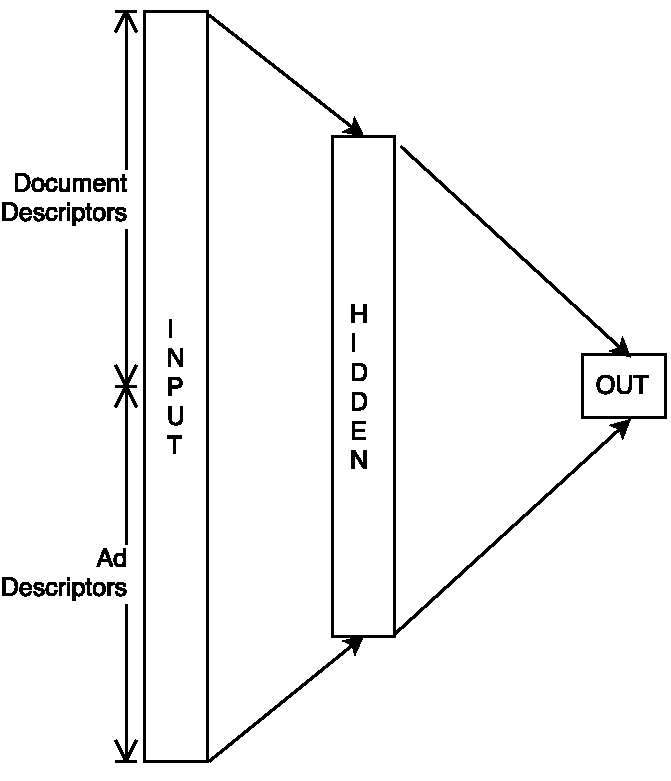
\includegraphics[scale=0.4]{Architecture}
% \end{floatrow}
\caption{Architecture}
\label{fig:architecture}
\end{figure}

% The second experiment involved more complicated feature engineering to make CTR predictions. Under the assumption that there must exist some representation of each document that describes its content, a correlation between the content of a user's current document to the content of an ad would likely increase the probability of that ad being clicked. To train a model to find this representation of content and compare it to the ad content, a shallow neural network was utilized. The neural network architecture had a single layer of 400 hidden units. This architecture was chosen over deeper models because \cite{mcmahan2013ad} noted that simpler models are dominating the CTR prediction community. It seems that relationships among the features were very simple, and the major challenge in CTR is feature engineering and selection. For this reason and time constraints, the 

\begin{center}
\begin{tabular}{c|ccc}
 &$\#$ Training&$\#$ Testing&Testing Accuracy \\\hline\hline
No PCA  & 80000  & 13000 & $93.3\%$ \\
PCA   & 80000 & 13000 & $95.82\%$\\
No PCA   & 120000 & 66776 &  $94.78\%$\\
PCA  & 120000  & 66776 & $95.71\%$\\
\end{tabular}
\end{center}


A single hidden layer neural network was selected to be the prime tool for prediction in these experiments. A cross-entropy loss and rectified linear transfers were used during training.
Due to the time constraints and the size of the dataset, the model was trained using a small set randomly sampled from the 83 million data points.  The above table shows the accuracy of 
each networks and training sets. By reducing the features through PCA the accuracy increased by almost $3\%$ and the added training samples also increased the accuracy. While the accuracy
looks impressive we found that in these sets approximately $80\%$ were not clicked. Our model does do better than just guessing not clicked, but could still use some improvement.

% Need some picture describing the neural network architecture.
% Would like to see some graph of the performance of the neural network
% A confusion matrix may look really nice here as well.


\section{Summary and Conclusions}

This paper proposed and tested two techniques for predicting the CTR given a users history and currently viewed document. The MLE provided a stepping stone in understanding the data
and performed adequately in predicting a user's clicks The neural network performed very well receiving $95.71\%$ accuracy, outperforming the MLE model significantly. While this is a 
good result, we suspect there is a lot of overfitting due to the lack of regularization used in training the network. In the future we would like to continue improving on the two models 
focusing on increasing the training and testing sets size as to create a more robust learned model. Also we would like to take advantage of the wealth of information contained in the 
document meta data and other portions of the larger dataset.


%------------------------------------------------
\phantomsection
\section*{Acknowledgments} % The \section*{} command stops section numbering
We must thank Outbrain for providing a vast and complicated dataset, and fear their monolithic approach to collecting vast swaths of user data.

\addcontentsline{toc}{section}{Acknowledgments} % Adds this section to the table of contents

%----------------------------------------------------------------------------------------
%	REFERENCE LIST
%----------------------------------------------------------------------------------------
\phantomsection
\bibliographystyle{unsrt}
\bibliography{report}

%----------------------------------------------------------------------------------------

\end{document}
